\chapter{State Of The Art}
  This chapter, after having introduced the concept of cognitive architecture, describes the main working instrument used for this work: \mbox{ACT-R,} the cognitive architecture and \mbox{OpenCV,} the computer vision library. 
  %% Cognitive Architecture
  \section{Cognitive Architecture}	
	A cognitive architecture is the implementation through computer simulation softwares \todo{controllare correttezza di softwares} of a theory about human cognition. The theory generally relies on a wide selection of human experimental data. The design of these architectures tries to simulate human intelligence in a humanlike way.
	
	\textit{"A cognitive architecture is not a single algorithm or method for solving a problem; rather, it is the task-independent infrastructure that brings an agent’s knowledge to bear on a problem in order to produce behavior"}~\cite{SoarCogArch2012}. A cognitive architecture alone can not solve any problem. In order to be able to do it, it needs to be supplied with the knowledge to perform it. The combination of an architecture and the knowledge necessary to solve a specific task is called \emph{model}. It is possible to create many models able to solve the same task. The specific knowledge is determined by the \emph{modeler} ~\cite{Sears2012}. 
	
	Another important feature of cognitive architectures is that they give the possibility to make comparison between the sequence of actions produced by the model and the ones produced by human beings when they try to solve the same task. In addition, the measured quantities can be not only qualitative ones, like the correctness of the goal, but also quantitative, as for example, the time necessary to complete a task. This gives the models the possibility to produce execution times, error rates and learning curves. Comparisons with human performances can be useful to evaluate the quality of model ~\cite{Sears2012}. 
	
	As the term \emph{infrastructure} suggests, cognitive architectures usually are built aggregating many software modules, most of which represent functions of the human brain. Anyway, there exist other modules, which coordinate the overall functioning and without which the whole architecture could not work. In the following section, which describes \emph{ACT-R}, the \emph{procedural module} is an example of such modules. In fact, it does not represent a function of the human being, though it is necessary to coordinate the communication between all the other modules. 
	
	Some architectures, can, in addition, include some \emph{learning mechanisms}. This can be the attempt to simulate the human memory system, thanks to which the behaviour of a human can be different after having experienced facts or consequences of a specific choice ~\cite{Sears2012}.
	
	
  %% ACT-R
  \section{ACT-R}
	\mbox{ACT-R}, that stands for \emph{Adaptive Control of Thought-Rational}, is a cognitive architecture that implements the homonym theory developed by John Robert Anderson, professor of psychology and computer science at Carnegie Mellon University. 
	\mbox{ACT-R} is a software written in Lisp and its models are written in a Lisp-like language. It is thought to have a modular structure so that it can be easily extended. The current version of the software is the 6.0. 
	
	The following section describes the differences between declarative and procedural memory. This is important because it is the basic theory on which ACT-R is founded. Then, after the definition of chunk and productions, the building blocks of ACT-R structure, you can find an overview on the architecture of the framework.
	
	\subsection{Declarative memory and procedural memory}
	In psychology, \emph{memory} is defined as the processes by which information is encoded, stored and retrieved ~\cite{baddeley2009memory}. 
	
	\mbox{ACT-R's} most important assumption about knowledge is based on Anderson's theory about memory. 
	Anderson divides memory into \emph{declarative} and \emph{procedural}. 
	
	Declarative memory refers to all the information that can be consciously recalled. This kind of knowledge comprehends facts and notions that human beings explicitly know. To call back this kind of information, there must be a conscious process by the human being. For this reason, this kind of memory is also called \emph{explicit}.
	
	In contrast, procedural memory refers to all that notions or skills that human beings have but which they learnt in an implicit way. Examples of this knowledge are, for example, driving, reading and writing. In this case, in order to call back this kind of information, the human being does not need a conscious process. That is why this kind of memory is also called \emph{implicit} ~\cite{anderson1976language}. 
	
	The following example is used to explain better how these two kinds of memory work. 
	When a person starts learning typewriting, an attempt he can make in the beginning is trying to memorize the layout of the keyboard. The aware knowledge of all the positions of the keys is the declarative memory. After having become a skilled typewriter, the same person will write quickly putting his fingers on the right keys and pushing them in the correct order, without thinking anymore about the positions of the keys on the keyboard. Moreover, if we ask him where the position of a certain character is on the keyboard, he will probably answer that he can not say it without looking at it. This is because, now, for this task he is using his procedural memory ~\cite{anderson1993rules}.
	
	\subsection{Chunks and productions}
	In \mbox{ACT-R}, declarative memory is represented by structures, called \emph{chunks}, and procedural memory  by rules, called \emph{productions}. Chunks and productions are the basic building blocks of an ACT-R model ~\cite{actr6refman}.
	
	The \emph{chunks} are data structures which are defined by their \emph{type} and their \emph{attribute list}. This is a tuple of pairs, each of which is made up by a fixed part and a variable part.
	The fixed part is the \emph{name} of the attribute and is called \emph{slot}.
	The variable part is the \emph{value} of the attribute.
% 	called \emph{slot} and is composed by the \emph{name} of the attribute, which is fixed for a certain chunk, and the \emph{value} of the attribute, which, instead, can assume different values. 
	Each chunk has also a \emph{name} but it is not considered to be a part of the chunk itself, as it does not exist in \mbox{ACT-R} theory. It is used only for convenience to reference the specific chunk when writing models. The chunk-types can be organized into hierarchies ~\cite{actr6refman}.
	
	The \emph{productions} are the \mbox{ACT-R} equivalent of functions. They define sequences of actions and can be fired only if a set of preconditions is satisfied. They can be represented as \emph{if-then} rules, where the \emph{if-part} is a set of conditions that must be true for the production to apply and the \emph{then-part} is the action of the production and consists of the operations the model should perform when the production is selected and used. 
	In general there could be some conflicts between productions. This happens when preconditions of two or more productions are satisfied at the same time. In these cases the production to be fired is the one with the highest \emph{utility value}. This is a numeric quantity which gives a priority measure. It can be set a priori by the modeler or learnt while the model is running ~\cite{actr6refman}.
	

	\subsection{Architecture}
	All the activities carried out by the human brain, like talking or moving, are performed by neurons located close together in a well defined and limited area of the cortex. Trying to imitate this "architecture", \mbox{ACT-R's} framework is structured in different \emph{modules}, each of which represents one specific function of the human brain ~\cite{actr6refman}. 
	
	Figure \ref{fig:modulesActr} shows the modular structure of ACT-R. In the picture you can see two groups of modules, separated by the \emph{procedural module} ~\cite{actr6refman}. 
	
	The first group comprehends \emph{visual}, \emph{aural}, \emph{manual } and \emph{vocal modules}. These let the model interact with the environment.
	The \emph{visual module} is responsible for recognizing objects in the visual scene and shifting the focus to them. Similarly, the \emph{aural module} identifies sounds and moves the attention to them. 
	The \emph{manual module} can move the virtual hands and perform actions like pressing the key on a keyboard or moving the mouse while the \emph{vocal module} controls the virtual voice ~\cite{actr6refman}.
	
	The other group comprehends \emph{goal module}, \emph{imaginal module} and \emph{declarative module}. These represent the internal information of the model.  
	The \emph{goal module} provides the system with the structure of the goal of the task, defined as a chunk. 
	The \emph{imaginal module} has to contain and update the current context relevant to the current task. 
	The \emph{declarative module} provides the model with a declarative memory, thus it stores the declarative chunks generated by the model and provides a mechanism for retrieving them ~\cite{actr6refman}. 
	
	Finally, the \emph{procedural module} is responsible of the communication and the coordination of all the other modules ~\cite{actr6refman}. 
	
	\begin{figure}[h]
	  \begin{center} 
	    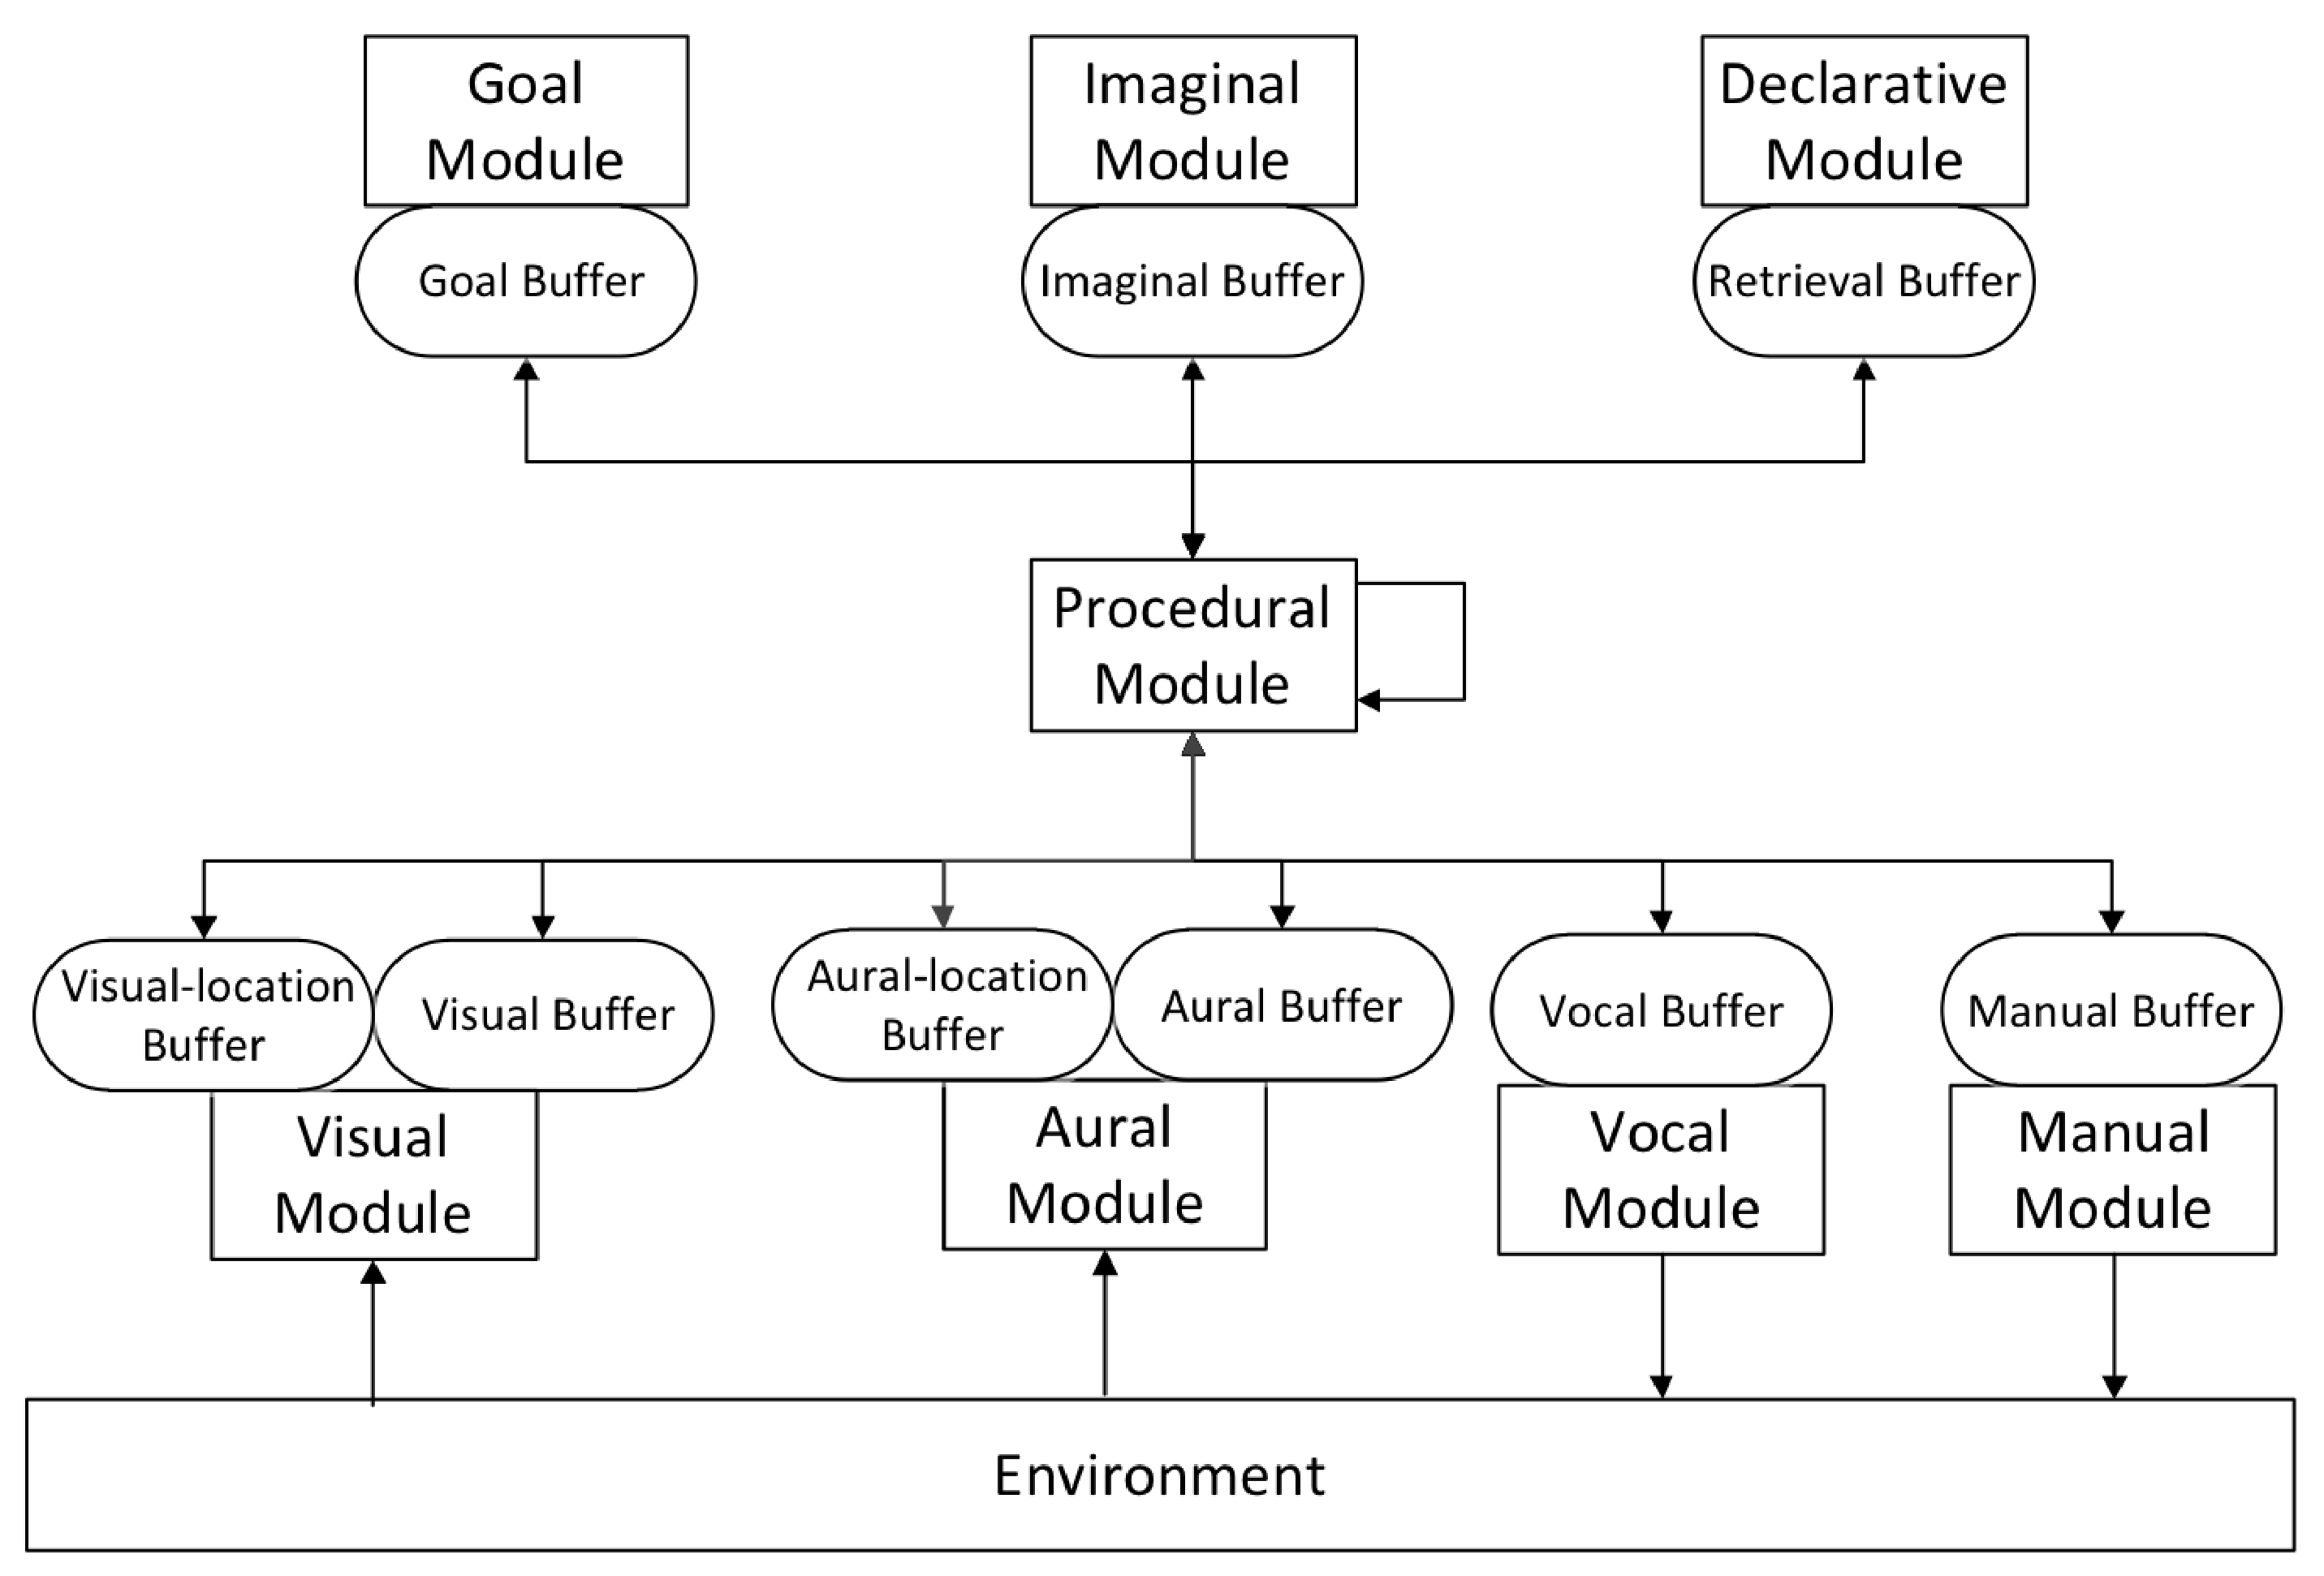
\includegraphics[scale=0.25]{images/ch_01/actr.eps}
	  \end{center} 
	  \caption{\textit{Structure of ACT-R.}}  
	  \label{fig:modulesActr}
	\end{figure}
	
	
	In fact, modules are independent of each other, they do not share variables or information. They can communicate with each other thanks to the \emph{buffers}, which represent the interfaces of a module towards the others. A module can have no buffers as well as one or more than one. The communication consists in exchanging chunks. Each module can read chunks from every buffer but it can make changes only to the chunks in its own buffers. Moreover each buffer can hold one chunk at a time ~\cite{actr6refman}. 

	Although modules usually work in a parallel way, their interactions can be only serial.
	There are two reasons for this limitation: the first one is that the structure of the buffers can hold only one chunk and the second one is that only one production can be fired at a time ~\cite{actr6refman}.
	
	
  %% OPENCV
  \section{OpenCV}
	\mbox{OpenCV}, an abbreviation that stands for \emph{Open Source Computer Vision}, is a computer vision library that was originally developed by Intel and, later on, by Willow Garage.
	It is a cross-platform library, released under a BSD license, thus it is free and open source. In the beginning it was developed in C and C++ and afterwards it was expanded by the addition of interfaces for Java and Python. \mbox{OpenCV} is designed for computational efficiency and with a strong focus on real-time applications. The version 2.4 has more than 2500 algorithms. The library has been used in many applications as, for example, mine inspection and robotics \cite{OpenCV:MainWebPage}. The following sections contain a brief history of the library and a list of its main features.
		
	\subsection*{History}
	The \mbox{OpenCV} Project started in 1999 as an Intel Reasearch initiative aimed to improve CPU intensive applications as a part of projects including real-time ray tracing and 3D display walls. The early goals of the project were developing optimized code for basic vision infrastructure, spreading this infrastructure to developers and making it portable and available for free, using a license that let the developers create both commercial and free applications.\newline
	The first alpha version was released to the public in 2000, followed by five beta versions between 2001 and 2005, which lead to version 1.0 in 2006. In 2008, the technology incubator Willow Garage begun supporting the project and, in the same year, version 1.1  was released.
	In October 2009, \mbox{OpenCV} 2.0 was released. It includes many improvements, such as a better C++ interface, more programming patterns, new functions and an optimization for multi-core architectures. According to the current \mbox{OpenCV} release plan, a new version of the library is delivered on a six-months basis. \cite{OpenCV:ChangeLogs}.
	
	\subsection*{Main Features}
	\mbox{OpenCV} offers a wide range of possibilities. First of all, it provides an easy way to manage image and video data types. It also offers functions to load, copy, edit, convert and store images and a basic graphical user interface that lets the developers handle keyboard and mouse and display images and videos. The library lets manipulate images even with matrix and vector algebra routines. It supports the most common dynamic data structures and offers many different basic image processing functions: filtering, edge and corner detection, color conversion, sampling and interpolation, morphological operations, histograms and image pyramids. Beyond this, it integrates many functions for structural analysis of the image, camera calibration, motion analysis and object recognition. \cite{Agam2006}.
